\documentclass{standalone}

\usepackage{tikz, xcolor}
\usetikzlibrary{folding,calendar}

\begin{document}


\sffamily\scriptsize
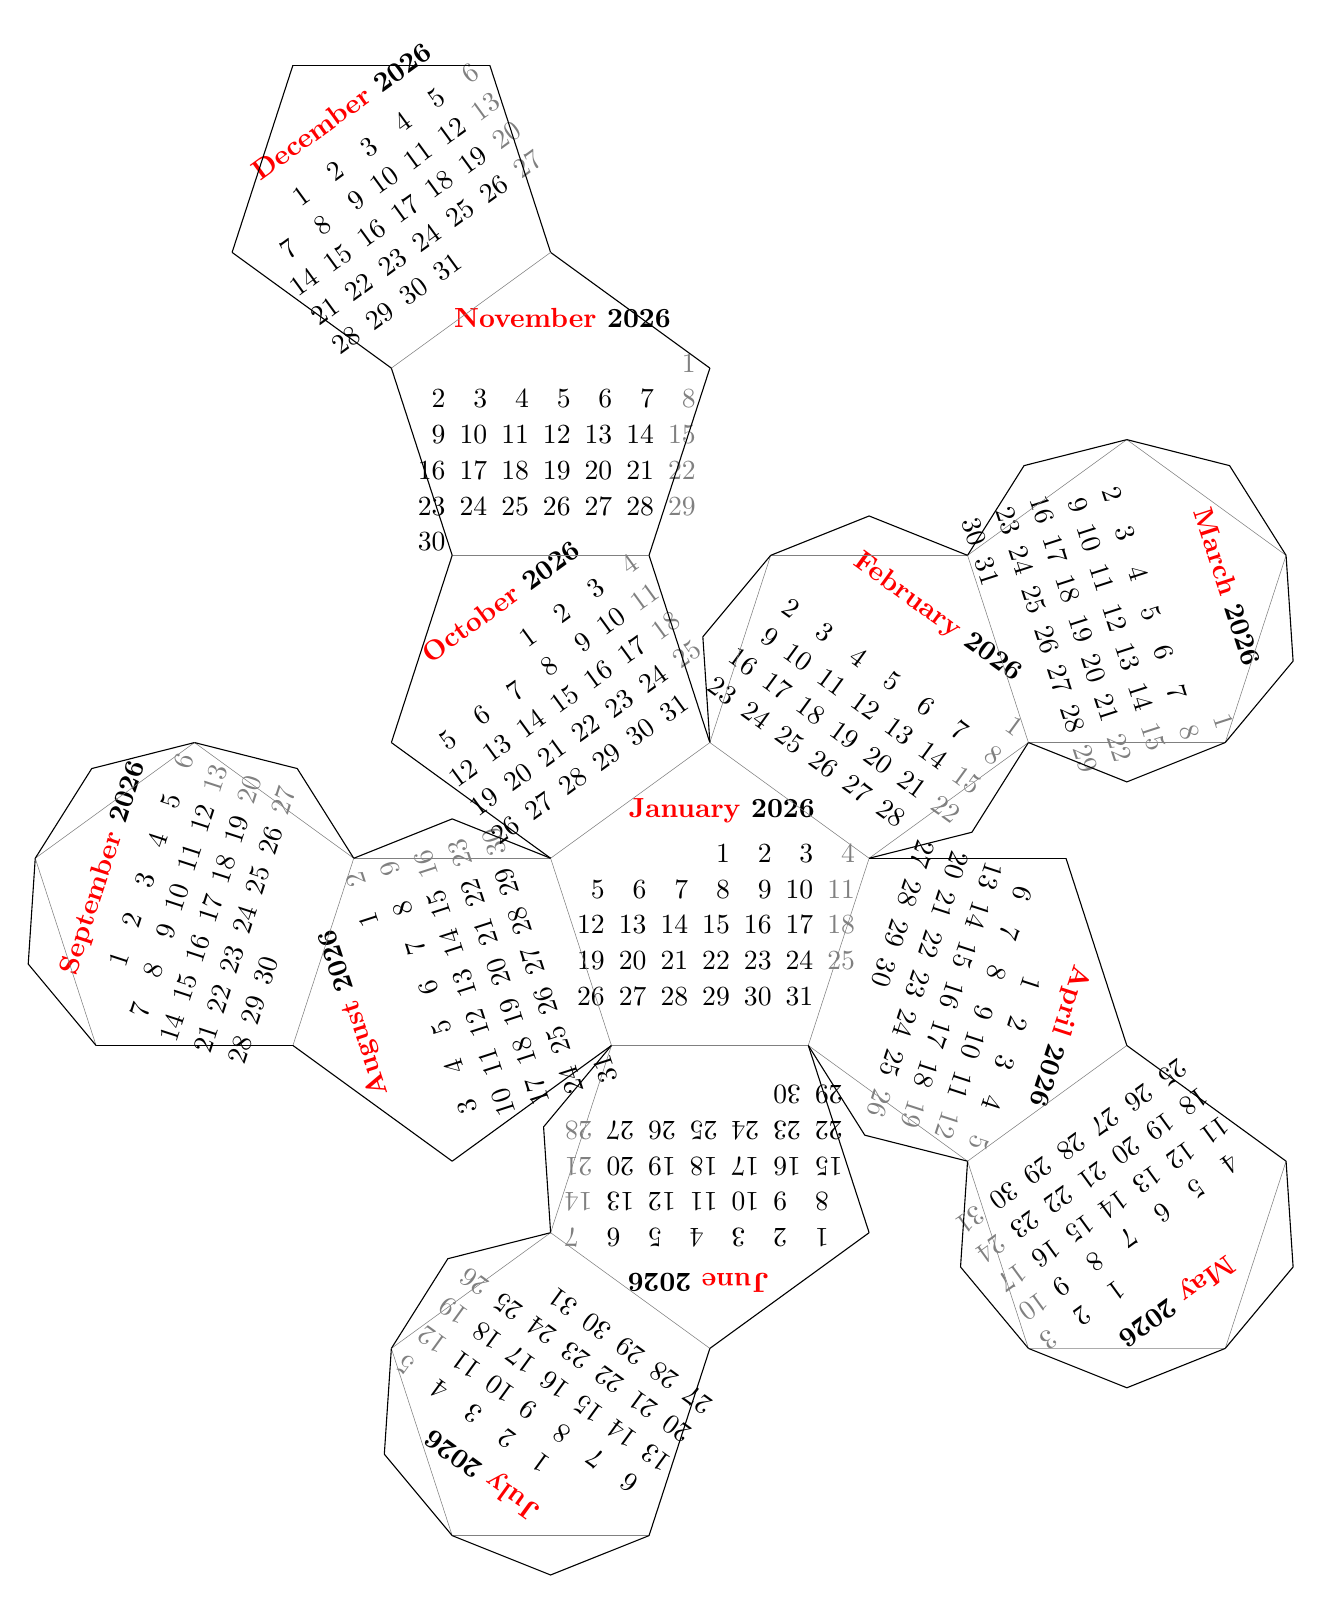
\begin{tikzpicture}[transform shape]
\tikzstyle{every calendar}=
[
    %Formats calendars and sets positions
    at={(-8ex,4ex)},
    week list,
    month label above centered,
    month text=\bfseries\textcolor{red}{\%mt} \%y0,
    if={(Sunday) [black!50]}
    ]
\tikzfoldingdodecahedron
[
    %Sets size of calendar
    folding line length=2.5cm,
    %Adds calendar image to each face
    face 1={ \calendar [dates=\the\year-01-01 to \the\year-01-last];},
    face 2={ \calendar [dates=\the\year-02-01 to \the\year-02-last];},
    face 3={ \calendar [dates=\the\year-03-01 to \the\year-03-last];},
    face 4={ \calendar [dates=\the\year-04-01 to \the\year-04-last];},
    face 5={ \calendar [dates=\the\year-05-01 to \the\year-05-last];},
    face 6={ \calendar [dates=\the\year-06-01 to \the\year-06-last];},
    face 7={ \calendar [dates=\the\year-07-01 to \the\year-07-last];},
    face 8={ \calendar [dates=\the\year-08-01 to \the\year-08-last];},
    face 9={ \calendar [dates=\the\year-09-01 to \the\year-09-last];},
    face 10={\calendar [dates=\the\year-10-01 to \the\year-10-last];},
    face 11={\calendar [dates=\the\year-11-01 to \the\year-11-last];},
    face 12={\calendar [dates=\the\year-12-01 to \the\year-12-last];},
];
\end{tikzpicture}

\end{document}